\section{Zur Programmierung verwendete Software}
Die Programmierung der Mikrocontroller wurde in \textit{PlatformIO} durchgeführt. 
Hierbei handelt es sich um eine Programmierumgebung, in welcher sich, ähnlich wie in der \textit{Arduino IDE}, eine Vielzahl von unterschiedlichen Prozessoren programmieren lassen.\\
Sie bietet nicht nur den Vorteil, über eine gut funktionierende Autovervollständigung zu Verfügen, sondern bietet auch (anders als die Verwendung eines reinen WINAVR Compilers, wie beispielsweise in der Eclipse) die Möglichkeit, \textit{Arduino.h} zu verwenden 
um den Programmcode nicht unnötig komplex ausführen zu müssen.

\newpage

\subsection{Visual Studio Code}
Wenngleich \textit{PlatformIO} in einer Reihe von Texteditoren zur Verfügung steht, wurde \textit{Visual Studio Code} von \textit{Microsoft} aufgrund seiner umfassenden Erweiterungsmöglichkeiten verwendet.\\
\href{https://code.visualstudio.com/}{Visual Studio Code Webseite}
\begin{figure}[h]
	\centering
	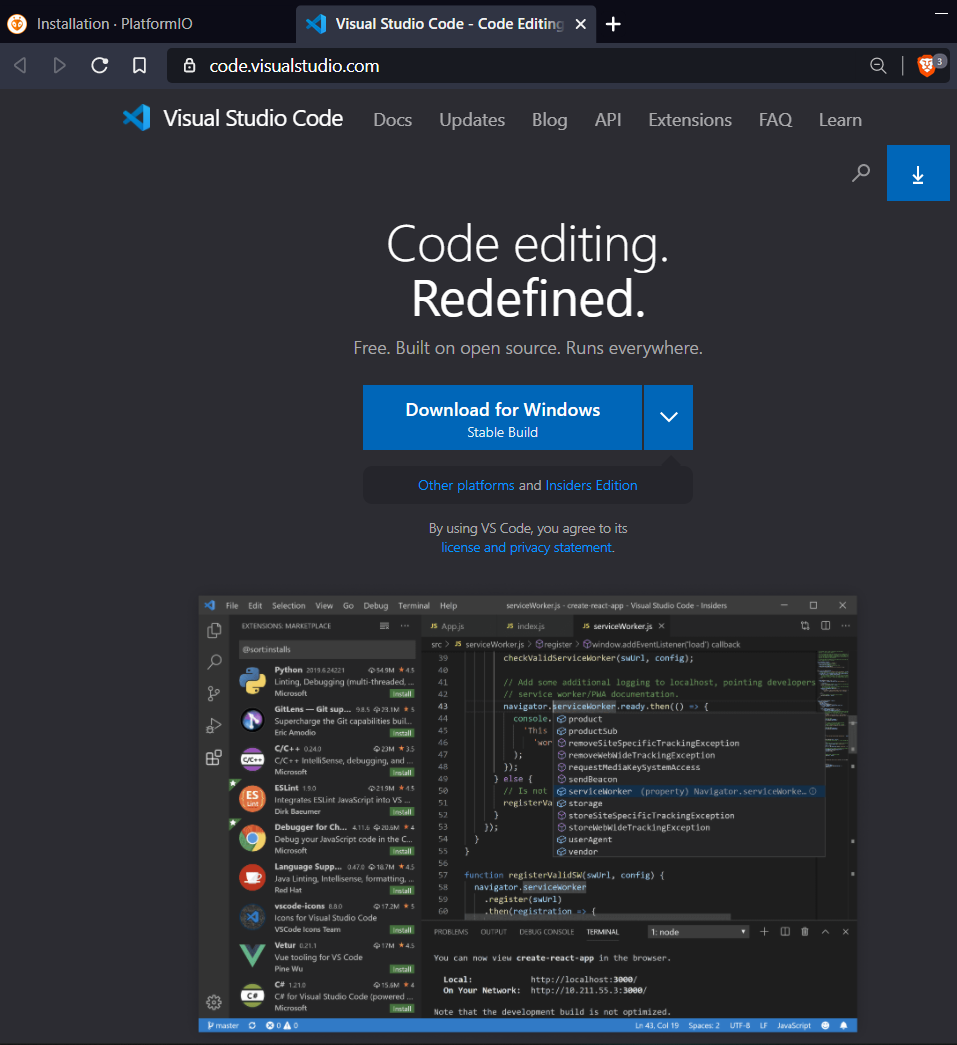
\includegraphics[width=0.85\textwidth]{bilder/Webseite_VSCode.png}
	\caption{Visual Studio Code Webseite}
\end{figure}

Visual Studio Code wird anschließend mit seiner Standard-Auswahl bei allen Abfragen installiert, weswegen hier auf eine genauere Dokumentation verzichtet wurde.

\newpage
\subsection{PlatformIO IDE}
Die Installation der Programmierumgebung \textit{PlatformIO IDE} erfolgt direkt über den in \textit{Visual Studio Code} integrierten Erweiterungs-Manager.\\
\href{https://platformio.org/install/ide?install=vscode}{PlatformIO Download Webseite}
\begin{figure}[h]
	\centering
	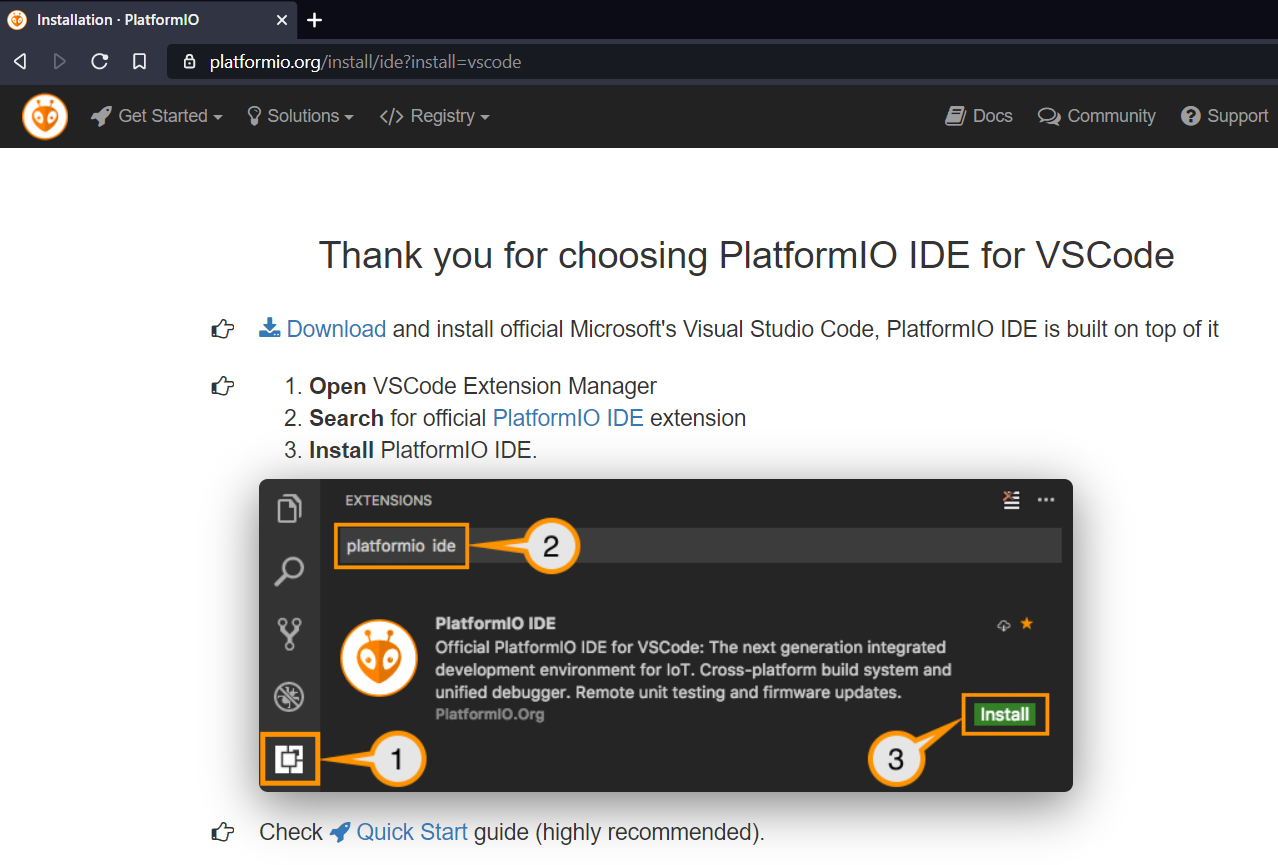
\includegraphics[width=0.8\textwidth]{bilder/Webseite_PlatformIO.png}
	\caption{PlatformIO Webseite}
\end{figure}

\textbf{Anmerkung:}\\
In neueren Versionen von Visual Studio Code ist das Icon des \textit{Extension Managers} nicht mehr das in obiger Abbildung gezeigte, sondern folgendes:

\includegraphics[align=t,width=0.8cm]{bilder/Icon_Extension_Manager.png}\\

Dieser Vorgang kann einige Minuten in Anspruch nehmen, und sollte am Ende zu einem \textit{Reload Window} auffordern. Danach ist die für die Diplomarbeit benötigte Software vollständig installiert und Einsatzbereit.\\

Video um den Einstieg in PlatformIO zu erleichtern: \href{https://youtu.be/JmvMvIphMnY?t=715}{Youtube-Tutorial zu PlatformIO}\\

\newpage